\documentclass[a4paper, 12pt]{article}
% for linebreaks and sectioning commands in german
\usepackage[ngerman]{babel}
% Encoding for German sonderzeichen
\usepackage[utf8]{inputenc}
% for size of borders etc.
\usepackage{geometry}
% for hyperlinks
\usepackage[hidelinks]{hyperref}
% for some nice pics
\usepackage{graphicx}
% for algorithm env
\usepackage{algpseudocode, algorithm}
% for math env
\usepackage{mathtools}
% caption
% \usepackage{caption}

% set size env
\geometry{a4paper,left=25mm,right=25mm, top=2cm, bottom=2cm}



\begin{document}

% Title Page
%%%%%%%%%%%%%%%%%%%%%%%%%%%%%%%%%%%%%%%%%
% University Assignment Title Page 
% LaTeX Template
% Version 1.0 (27/12/12)
%
% This template has been downloaded from:
% http://www.LaTeXTemplates.com
%
% Original author:
% WikiBooks (http://en.wikibooks.org/wiki/LaTeX/Title_Creation)
%
% License:
% CC BY-NC-SA 3.0 (http://creativecommons.org/licenses/by-nc-sa/3.0/)
% 
% Instructions for using this template:
% This title page is capable of being compiled as is. This is not useful for 
% including it in another document. To do this, you have two options: 
%
% 1) Copy/paste everything between \begin{document} and \end{document} 
% starting at \begin{titlepage} and paste this into another LaTeX file where you 
% want your title page.
% OR
% 2) Remove everything outside the \begin{titlepage} and \end{titlepage} and 
% move this file to the same directory as the LaTeX file you wish to add it to. 
% Then add %%%%%%%%%%%%%%%%%%%%%%%%%%%%%%%%%%%%%%%%%
% University Assignment Title Page 
% LaTeX Template
% Version 1.0 (27/12/12)
%
% This template has been downloaded from:
% http://www.LaTeXTemplates.com
%
% Original author:
% WikiBooks (http://en.wikibooks.org/wiki/LaTeX/Title_Creation)
%
% License:
% CC BY-NC-SA 3.0 (http://creativecommons.org/licenses/by-nc-sa/3.0/)
% 
% Instructions for using this template:
% This title page is capable of being compiled as is. This is not useful for 
% including it in another document. To do this, you have two options: 
%
% 1) Copy/paste everything between \begin{document} and \end{document} 
% starting at \begin{titlepage} and paste this into another LaTeX file where you 
% want your title page.
% OR
% 2) Remove everything outside the \begin{titlepage} and \end{titlepage} and 
% move this file to the same directory as the LaTeX file you wish to add it to. 
% Then add %%%%%%%%%%%%%%%%%%%%%%%%%%%%%%%%%%%%%%%%%
% University Assignment Title Page 
% LaTeX Template
% Version 1.0 (27/12/12)
%
% This template has been downloaded from:
% http://www.LaTeXTemplates.com
%
% Original author:
% WikiBooks (http://en.wikibooks.org/wiki/LaTeX/Title_Creation)
%
% License:
% CC BY-NC-SA 3.0 (http://creativecommons.org/licenses/by-nc-sa/3.0/)
% 
% Instructions for using this template:
% This title page is capable of being compiled as is. This is not useful for 
% including it in another document. To do this, you have two options: 
%
% 1) Copy/paste everything between \begin{document} and \end{document} 
% starting at \begin{titlepage} and paste this into another LaTeX file where you 
% want your title page.
% OR
% 2) Remove everything outside the \begin{titlepage} and \end{titlepage} and 
% move this file to the same directory as the LaTeX file you wish to add it to. 
% Then add \input{./title_page_1.tex} to your LaTeX file where you want your
% title page.
%
%%%%%%%%%%%%%%%%%%%%%%%%%%%%%%%%%%%%%%%%%

%----------------------------------------------------------------------------------------
%	PACKAGES AND OTHER DOCUMENT CONFIGURATIONS
%----------------------------------------------------------------------------------------

\begin{titlepage}

\newcommand{\HRule}{\rule{\linewidth}{0.5mm}} % Defines a new command for the horizontal lines, change thickness here

\center % Center everything on the page
 
%----------------------------------------------------------------------------------------
%	HEADING SECTIONS
%----------------------------------------------------------------------------------------

\textsc{\LARGE Universität Osnabrück}\\[1.5cm] % Name of your university/college
\textsc{\Large Seminar Verteilte Systeme\\\normalsize Wintersemester 14/15}\\[0.5cm] % Major heading such as course name
% \textsc{\large Seminarausarbeitung}\\[0.5cm] % Minor heading such as course title
\textsc{\large Prof. Nils Aschenbruck}\\[0.5cm] % Minor heading such as course title

%----------------------------------------------------------------------------------------
%	TITLE SECTION
%----------------------------------------------------------------------------------------

\HRule \\[0.4cm]
{ \huge \bfseries Opportunistische Netze\\\Large Anwendungen, Protokolle und Modelle}\\[0.4cm] % Title of your document
\HRule \\[1.5cm]
 
%----------------------------------------------------------------------------------------
%	AUTHOR SECTION
%----------------------------------------------------------------------------------------

\begin{minipage}{0.4\textwidth}
\begin{flushleft} \large
\emph{Author:}\\
Christian \textsc{Heiden}\\
\href{mailto:cheiden@uos.de}{cheiden@uos.de}\\
(945303)
\end{flushleft}
\end{minipage}
~
\begin{minipage}{0.4\textwidth}
\begin{flushright} \large
\emph{Supervisor:} \\
Matthias \textsc{Schwamborn} % Supervisor's Name
\end{flushright}
\end{minipage}\\[4cm]

% If you don't want a supervisor, uncomment the two lines below and remove the section above
%\Large \emph{Author:}\\
%John \textsc{Smith}\\[3cm] % Your name

%----------------------------------------------------------------------------------------
%	DATE SECTION
%----------------------------------------------------------------------------------------

{\large \today}\\[3cm] % Date, change the \today to a set date if you want to be precise

%----------------------------------------------------------------------------------------
%	LOGO SECTION
%----------------------------------------------------------------------------------------

% \includegraphics{logo.png}\\[1cm] % Include a department/university logo - this will require the graphicx package
 
%----------------------------------------------------------------------------------------

\vfill % Fill the rest of the page with whitespace

\end{titlepage} to your LaTeX file where you want your
% title page.
%
%%%%%%%%%%%%%%%%%%%%%%%%%%%%%%%%%%%%%%%%%

%----------------------------------------------------------------------------------------
%	PACKAGES AND OTHER DOCUMENT CONFIGURATIONS
%----------------------------------------------------------------------------------------

\begin{titlepage}

\newcommand{\HRule}{\rule{\linewidth}{0.5mm}} % Defines a new command for the horizontal lines, change thickness here

\center % Center everything on the page
 
%----------------------------------------------------------------------------------------
%	HEADING SECTIONS
%----------------------------------------------------------------------------------------

\textsc{\LARGE Universität Osnabrück}\\[1.5cm] % Name of your university/college
\textsc{\Large Seminar Verteilte Systeme\\\normalsize Wintersemester 14/15}\\[0.5cm] % Major heading such as course name
% \textsc{\large Seminarausarbeitung}\\[0.5cm] % Minor heading such as course title
\textsc{\large Prof. Nils Aschenbruck}\\[0.5cm] % Minor heading such as course title

%----------------------------------------------------------------------------------------
%	TITLE SECTION
%----------------------------------------------------------------------------------------

\HRule \\[0.4cm]
{ \huge \bfseries Opportunistische Netze\\\Large Anwendungen, Protokolle und Modelle}\\[0.4cm] % Title of your document
\HRule \\[1.5cm]
 
%----------------------------------------------------------------------------------------
%	AUTHOR SECTION
%----------------------------------------------------------------------------------------

\begin{minipage}{0.4\textwidth}
\begin{flushleft} \large
\emph{Author:}\\
Christian \textsc{Heiden}\\
\href{mailto:cheiden@uos.de}{cheiden@uos.de}\\
(945303)
\end{flushleft}
\end{minipage}
~
\begin{minipage}{0.4\textwidth}
\begin{flushright} \large
\emph{Supervisor:} \\
Matthias \textsc{Schwamborn} % Supervisor's Name
\end{flushright}
\end{minipage}\\[4cm]

% If you don't want a supervisor, uncomment the two lines below and remove the section above
%\Large \emph{Author:}\\
%John \textsc{Smith}\\[3cm] % Your name

%----------------------------------------------------------------------------------------
%	DATE SECTION
%----------------------------------------------------------------------------------------

{\large \today}\\[3cm] % Date, change the \today to a set date if you want to be precise

%----------------------------------------------------------------------------------------
%	LOGO SECTION
%----------------------------------------------------------------------------------------

% \includegraphics{logo.png}\\[1cm] % Include a department/university logo - this will require the graphicx package
 
%----------------------------------------------------------------------------------------

\vfill % Fill the rest of the page with whitespace

\end{titlepage} to your LaTeX file where you want your
% title page.
%
%%%%%%%%%%%%%%%%%%%%%%%%%%%%%%%%%%%%%%%%%

%----------------------------------------------------------------------------------------
%	PACKAGES AND OTHER DOCUMENT CONFIGURATIONS
%----------------------------------------------------------------------------------------

\begin{titlepage}

\newcommand{\HRule}{\rule{\linewidth}{0.5mm}} % Defines a new command for the horizontal lines, change thickness here

\center % Center everything on the page
 
%----------------------------------------------------------------------------------------
%	HEADING SECTIONS
%----------------------------------------------------------------------------------------

\textsc{\LARGE Universität Osnabrück}\\[1.5cm] % Name of your university/college
\textsc{\Large Seminar Verteilte Systeme\\\normalsize Wintersemester 14/15}\\[0.5cm] % Major heading such as course name
% \textsc{\large Seminarausarbeitung}\\[0.5cm] % Minor heading such as course title
\textsc{\large Prof. Nils Aschenbruck}\\[0.5cm] % Minor heading such as course title

%----------------------------------------------------------------------------------------
%	TITLE SECTION
%----------------------------------------------------------------------------------------

\HRule \\[0.4cm]
{ \huge \bfseries Opportunistische Netze\\\Large Anwendungen, Protokolle und Modelle}\\[0.4cm] % Title of your document
\HRule \\[1.5cm]
 
%----------------------------------------------------------------------------------------
%	AUTHOR SECTION
%----------------------------------------------------------------------------------------

\begin{minipage}{0.4\textwidth}
\begin{flushleft} \large
\emph{Author:}\\
Christian \textsc{Heiden}\\
\href{mailto:cheiden@uos.de}{cheiden@uos.de}\\
(945303)
\end{flushleft}
\end{minipage}
~
\begin{minipage}{0.4\textwidth}
\begin{flushright} \large
\emph{Supervisor:} \\
Matthias \textsc{Schwamborn} % Supervisor's Name
\end{flushright}
\end{minipage}\\[4cm]

% If you don't want a supervisor, uncomment the two lines below and remove the section above
%\Large \emph{Author:}\\
%John \textsc{Smith}\\[3cm] % Your name

%----------------------------------------------------------------------------------------
%	DATE SECTION
%----------------------------------------------------------------------------------------

{\large \today}\\[3cm] % Date, change the \today to a set date if you want to be precise

%----------------------------------------------------------------------------------------
%	LOGO SECTION
%----------------------------------------------------------------------------------------

% \includegraphics{logo.png}\\[1cm] % Include a department/university logo - this will require the graphicx package
 
%----------------------------------------------------------------------------------------

\vfill % Fill the rest of the page with whitespace

\end{titlepage}

% Table of Contents
\pagenumbering{roman}
\tableofcontents
\newpage
\pagenumbering{arabic}
% Abstract
% \begin{abstract}

% \end{abstract}


% LEITFRAGEN
% Was sind opportunistische Netze (OppNets) und welche Untertypen gibt es?
% Wo liegen die besonderen Herausforderungen bei OppNets?
% In welchen Anwendungsgebieten finden OppNets Verwendung?
% Welche Arten von Forwarding-Protokollen gibt es fuer OppNets und worin unterscheiden sie sich?
% Welche Modelle sind im Kontext der Leistungsbewertung von OppNets besonders relevant und worin liegen deren Vor- und Nachteile?
% Was sind aktuelle und offene Probleme/Fragestellungen?


% EIGENE FRAGEN
% Wie lange soll der Vortrag werden? 30 Vortrag + 15 Diskussion
% Wieviele Seiten? 10

\section{Einleitung}
% motivation über manet und 
% jeder hat mobile endgeräte
% delays!

%%%%%%%%%%%%%% OLD
% Es gibt eine Vielzahl an verschiedenen Netzwerktopologien. Das Internet stellt eine Netzwerktopologie dar, in welcher alle (Knoten) direkt, über eine Infrastruktur miteinander kommunizieren können. Direkt bedeutet, dass es einen klar definierten Weg entlang einer festen Infrastruktur vom Startknoten zum Zielknoten gibt. Mit einer festen Infrastruktur ist gemeint, dass bestimmte Knoten in dem Netzwerk ausschließlich für das Überbringen von Nachrichten zuständig sind. Als Beispiel betrachte man einen Client, welcher eine Nachricht über (mehrere) Router zu einem Server sendet.
%%%%%%%%%%%%%% OLD


% HIER MEHR AN DEM ELSEVIER PAPER ORIENTIEREN
% es muss Manets besser von OppNets abgehoben werden (umgekehrt bzw.)
% OppNets sind manets, aber (achtung elsevier!) haben zwei besondere Charakterisiken:
% store-carry-forward paradigm und long end-to-end delay, weil keine direkte Verbindung besteht (bei Manets könnte das nämlich gegeben sein :-) )

% auch noch von kontakten sprechen...
%%%%%%%%%%%%%% OLD
%Diese Topologie zeichnet sich also (unter anderem) durch seine feste Infrastruktur und direkten Kommunikationswegen aus. Netzwerktopologien ohne diese beiden Aspekte werden als opportunistische Netze (OppNets) bezeichnet. 
% Das Fehlen der festen Infrastruktur, wird dadurch gelöst, dass jeder Teilnehmer (Knoten) in dem Netzwerk zugleich Client als auch Router darstellt. Verbindungen zwischen den Knoten finden also ad-hoc statt, das heißt Ende-zu-Ende. 
% Da Endgeräte in einem Netzwerk mobiler Natur sind (Handys, Laptops, etc.), ergibt sich eine mobile, dynamische Infrastruktur, welche ein herkömmliches Routing vor Probleme stellt. Es steht beim Versenden einer Nachricht nicht fest, welcher Weg zum Ziel führen wird, denn es gibt in der Regel keine aufrechte Verbindung zum Ziel, bzw. es kann nicht vorhergesagt werden, wie und ob sich die Struktur des Netzwerks verändern wird während des Sendens.
%%%%%%%%%%%%%%% OLD

Mobile Endgeräte wie Handys, Tablets oder Laptops sind immer populärer geworden. Die meisten dieser Geräte verfügen über drathlose Kommunikationsmöglichkeiten, wie Bluetooth, W-Lan, Mobilfunknetzanbindung und vielem mehr. Zusätzlich werden Akkulaufzeit, Speicherkapazität, Kommunikationsqualität, etc. permanent verbessert. Dies ermöglicht die Nutzung einer Klasse von Anwendungen, welche auf dem direkten Kontakt einzelner Endgeräten basiert. Ein \emph{Kontakt} ist definiert, als eine \emph{one-Hop}-Verbindung zweier Endgeräte, z.B. via Bluetooth, sodass ein Datenaustausch auf direktem Weg, also ohne Umwege über eine dritte Knoten, stattfinden kann. Dieser Verbindungstyp wird auch als \emph{ad-hoc} Verbindung bezeichnet.

Eine Klasse von Anwendungen in denen Endgeräte Daten ad-hoc verschicken sind sogenannte \emph{MANET}s (\emph{mobile ad hoc networks}) \cite[p.~2]{zeng2011multihop}. Einige (häufig die meisten, bis alle) Knoten eines MANETs sind frei beweglich, sodass deren Verbindungen zu anderen Knoten häufig wechseln können. Außerdem fungieren die Knoten eines MANETS sowohl als Sender, als auch als Router. Denn sobald eine Nachricht von Knoten $A$ zu Knoten $B$ verschickt werden soll, kann es passieren, dass es nie zu einem Kontakt zwischen $A$ und $B$ kommt. Folglich muss die Nachricht, über eine Menge von Knoten geleitet werden um schlussendlich bei Knoten $B$ anzugelangen.

Wenn die Zeitspanne zwischen Verschicken und Ankommen einer Nachricht groß ist, und das Prinzip des Forwardings innerhalb des Netzes nach dem store-carry-forward-Prinzip arbeitet, so bezeichnet man ein MANET auch als opportunistisches Netzwerk (\emph{OppNet}) \cite{Mota20145}.
Erstgenannte Eigenschaft wird auch \emph{end-to-end-delay} genannt.
Die Bezeichnung \emph{opportunistisch} leitet sich aus dem englischen Begriff \emph{opportunity} (Möglichkeit, Chance) ab und bedeutet, dass Knoten eines OppNets die auftretenden Kontakte als Chance sehen ihre Daten weiterzuleiten.
Anhand des bereits erwähnten \emph{store-carry-forward}-Prinzips, sollen im Folgenden die Grundlagen des Informationsaustauschs innerhalb eines OppNets erläutert werden:

Kommt es zu einem Kontakt zweier Knoten, tauschen sie in irgendeiner Form Informationen aus. Da beide Knoten, sowohl Sender als auch Router darstellen, speichern sie auch Informationen für andere Knoten ab. Durch ihre Mobilität, tragen sie also diese Informationen an andere Orte, auf deren Wegen es zu weiteren Kontakten kommen kann. Schlussendlich ist es möglich, dass so weitergeleitete Informationen, bei dem jeweiligen Zielknoten ankommen.
Eine Herausforderung in OppNets ist es, eine Strategie zu finden, welche Nachrichten so versendet, dass das Ziel erreicht wird. Durch die Mobilität einzelner Knoten, ist die Topologie des Netzes veränderlich und es fällt schwer  Aussagen über zukünftige Netzwerkzustände und damit verbundene Routen zu treffen.

Diese Ausarbeitung soll dem Leser einen Überblick über das Feld der OppNets geben. Zu Beginn werden zwei Anwendungen besprochen (Kapitel \ref{sec:applications}), in denen OppNets genutzt werden. Anschließend wird eine Einführung in die existierenden Forwarding-Protokolle gegeben (Kapitel \ref{sec:forwarding}) und es werden exemplarisch drei Protokolle vorgestellt. Daraufhin wird dem Leser ein Einblick in die zur Bewertung der Protokolle genutzten Simulationsmodelle gegeben (Kapitel \ref{sec:simulation}). 
% Weitergehend werden Probleme in der Umsetzung von OppNets besprochen (\ref{sec:problems})???.
In Abschnitt \ref{sec:conclusion} werden die in der Ausarbeitung besprochenen Inhalte zusammengefasst.


\section{Anwendungsgebiete}
\label{sec:applications}
%%%%%%%%%%%%%% OLD
% OppNets finden vor allem in Gebieten Anwendung, in denen eine Netzabdeckung aufgrund der Lage des Netzwerkes oder gewisser technischer Gegebenheiten nicht möglich ist. Im Folgenden werden zwei Projekte vorgestellt.
%%%%%%%%%%%%%% OLD
Generell eignen sich Opportunistische Netze in Situationen, wo es zu langen kontaktlosen Zeiten zwischen Knoten kommt und diese bei Kontakt in der Lage sind, Daten ad-hoc miteinander auszutauschen.
Beispielsweise gibt es Szenarien, in denen Autos die Knoten eines Netzwerkes darstellen und durch Kontakte mit anderen, z.B. entgegenkommenden, Autos Informationen über Wetter oder Straßenverhältnisse austauschen. Diese Netze werden auch als \emph{VANET}s (\emph{vehicular ad hoc networks}) bezeichnet \cite{Mota20145}.
Weitere Anwendungsgebiete sind Umgebungen in denen es keine Alternative zu opportunistischen Ansätzen gibt, weil es beispielsweise keine Anbindung an Mobilfunknetze gibt oder ständige Verbindungen aufgrund von Energieknappheit nicht möglich sind. Solche Umgebungen werden auch als \emph{challenged environments} bezeichnet \cite{Mota20145}.
Im Folgenden werden exemplarisch zwei weitere Szenarien tiefergehend vorgestellt, in denen OppNets zur Anwendung kommen.

% ZebraNet project
\subsection{ZebraNet}
\label{sec:applications:zebranet}
Ein Anwendungsgebiet ist das Beobachten von Tierverhalten. 
Beim \emph{ZebraNet} Projekt \cite{juang2002energy} wurden Zebras Geräte angelegt, welche als Knoten in einem Netz fungieren sollten. Die Umgebung, in der das Experiment stattfand, lässt sich in die Gruppe der challenging environments einordnen. Das Ziel war die Analyse ihrer Bewegungsmuster. Die Geräte verfügten über GPS, einem solar-betriebenen Akku, Flash-Speicher, einer kleinen CPU und Hardware zur Datenübertragung an benachbarte Geräte. Gesammelte Daten sollten an ein Auto, die sogenannte \emph{Base-Station}, übertragen werden, welches in gewissen Zeitabständen in Radio-Empfangsreichweite an den Zebras vorbeifuhr. Die Base-Station stellte das endgültige Ziel einer jeden Nachricht dar.

Dadurch ergibt sich die erste Herausforderung dieses Szenarios: Es ist nicht klar, ob ein Tier jemals Kontakt zur Base-Station haben wird.
Hierzu müssen Protokolle entwickelt werden, welche dafür sorgen, dass Nachrichten trotzdem an einer Base-Station ankommen, ohne, dass ein Kontakt zwischen Gerät und Base-Station jemals stattgefunden hat.
Weitere Herausforderungen sind limitierte Verfügbarkeit von Speicher und Energie, welche ein simples Fluten der Nachrichten an benachbarte Knoten auschließt.

\subsection{Haggle Project}
\label{sec:applications:haggle}
Im Rahmen des Haggle Project \cite{haggleProj} wurde eine Software erstellt, welche Nutzer auf ihren Smartphones installieren können. Die Idee ist der Austausch von Inhalten, abhängig von den Interessen der User. Dazu gibt der Nutzer seine eigenen Interessen an und versieht seine Inhalte mit Schlüsselwörtern.

Kommt es zu einem Kontakt zwischen zwei Nutzern, welche die Haggle-Software installiert haben, so findet ein Austausch der Daten statt, die den Interessen des anderen Users entsprechen.
Kontakte zwischen Smartphones finden auf Basis von Bluetooth oder W-Lan statt.
Hier ist zu beachten, dass Sender und Empfänger einer Nachricht immer die Beteiligten eines Kontakts sind, sodass ein Forwarding über mehrere Knoten nicht nötig ist.

Eine Herausforderung des Haggle Projekts ist die geringe Knotendichte des Netzwerks, da die Software nicht sehr populär ist. Als weitere Schwierigkeit ist die meist begrenzte Energieverfügbarkeit zu bennenen. Durch die ständigen Versuche Verbindungen an Schnittstellen wie Bluetooth oder W-Lan aufrecht zu erhalten, wird der Energieverbrauch des Endgeräts mitunter enorm angehoben.

\section{Forwarding-Protokolle}
\label{sec:forwarding}
Wegfindung stellt in opportunistischen Netzen die wohl größte Herausforderung dar.
Betrachtet man die Route einer Nachricht, als Pfad entlang von Routerknoten von einem Startknoten (Sender) zu einem Zielknoten (Empfänger), so lässt sich für Netzwerke wie z.B. dem Internet mit einer vergleichsweise hohen Wahrscheinlichkeit sagen, entlang welcher Knoten Nachrichten verschickt werden müssen, sodass sie ihr Ziel erreichen. Dies wird unter anderem mithilfe von Routingtabellen realisiert.

OppNets hingegen arbeiten mit der Annahme, dass theoretisch alle Knoten des Netzwerks mobil sein können, wodurch ein Einsatz von klassischen Routingtabellen in vielen Fällen nicht realisierbar ist.
Daher verwenden OppNets meist Verfahren, welche den nächsten Hop mit einer gewissen Wahrscheinlichkeit als zielführend bewerten. Manche Forwarding Strategien verwenden \emph{flooding}-Ansätze um die Wahrscheinlichkeit des Erreichens des Ziel zu erhöhen. Andere Strategien basieren auf Mustererkennung von Meta-Informationen wie z.B. vergangener Aufenthaltsorte, um die Wahrscheinlichkeit eines zielführenden nächsten Knotens zu schätzen.

Auf den Begriff \emph{Routing} wird hier absichtlich verzichtet, da dieser impliziert, dass eine konkrete Route entlang von Knoten beim erstmaligen Versenden einer Nachricht bekannt ist. Stattdessen werden Protokolle opportunistischer Netze allgemein als Forwarding-Protokolle bezeichnet (\cite[p.10]{Mota20145}).
\\\\
Nach \cite{Mota20145} werden Protokolle in drei Kategorien unterteilt:
\begin{description}
	\item [ohne Kontext]\hfill \\
	Kontextlose Protokolle wählen den nächsten Hop ohne auf Berechnung von Meta-Informationen zurückzugreifen. Diese Protokolle arbeiten meist mit Zufallskomponenten.
	\item [partieller Kontext]\hfill \\
	Protokolle mit partiellem Kontext beziehen relativ einfach erstellbare Netzwerkinformationen wie Kontakthistorien mit in die Wegfindung ein.
	\item [voller Kontext]\hfill \\
	Protokolle mit vollem Kontext stellen ein komplexes Modell der Knotennachbarschaften auf, sodass daraus Schlüsse gezogen werden können, welcher Knoten sich besser als potenzieller nächster Hop eignet als andere.
\end{description}
Im Folgenden wird zu jeder dieser Kategorien jeweils ein Beispiel gegeben und erklärt.

\subsection{Ohne Kontext - Epidemic}
\begin{figure}[H]
    \centering
    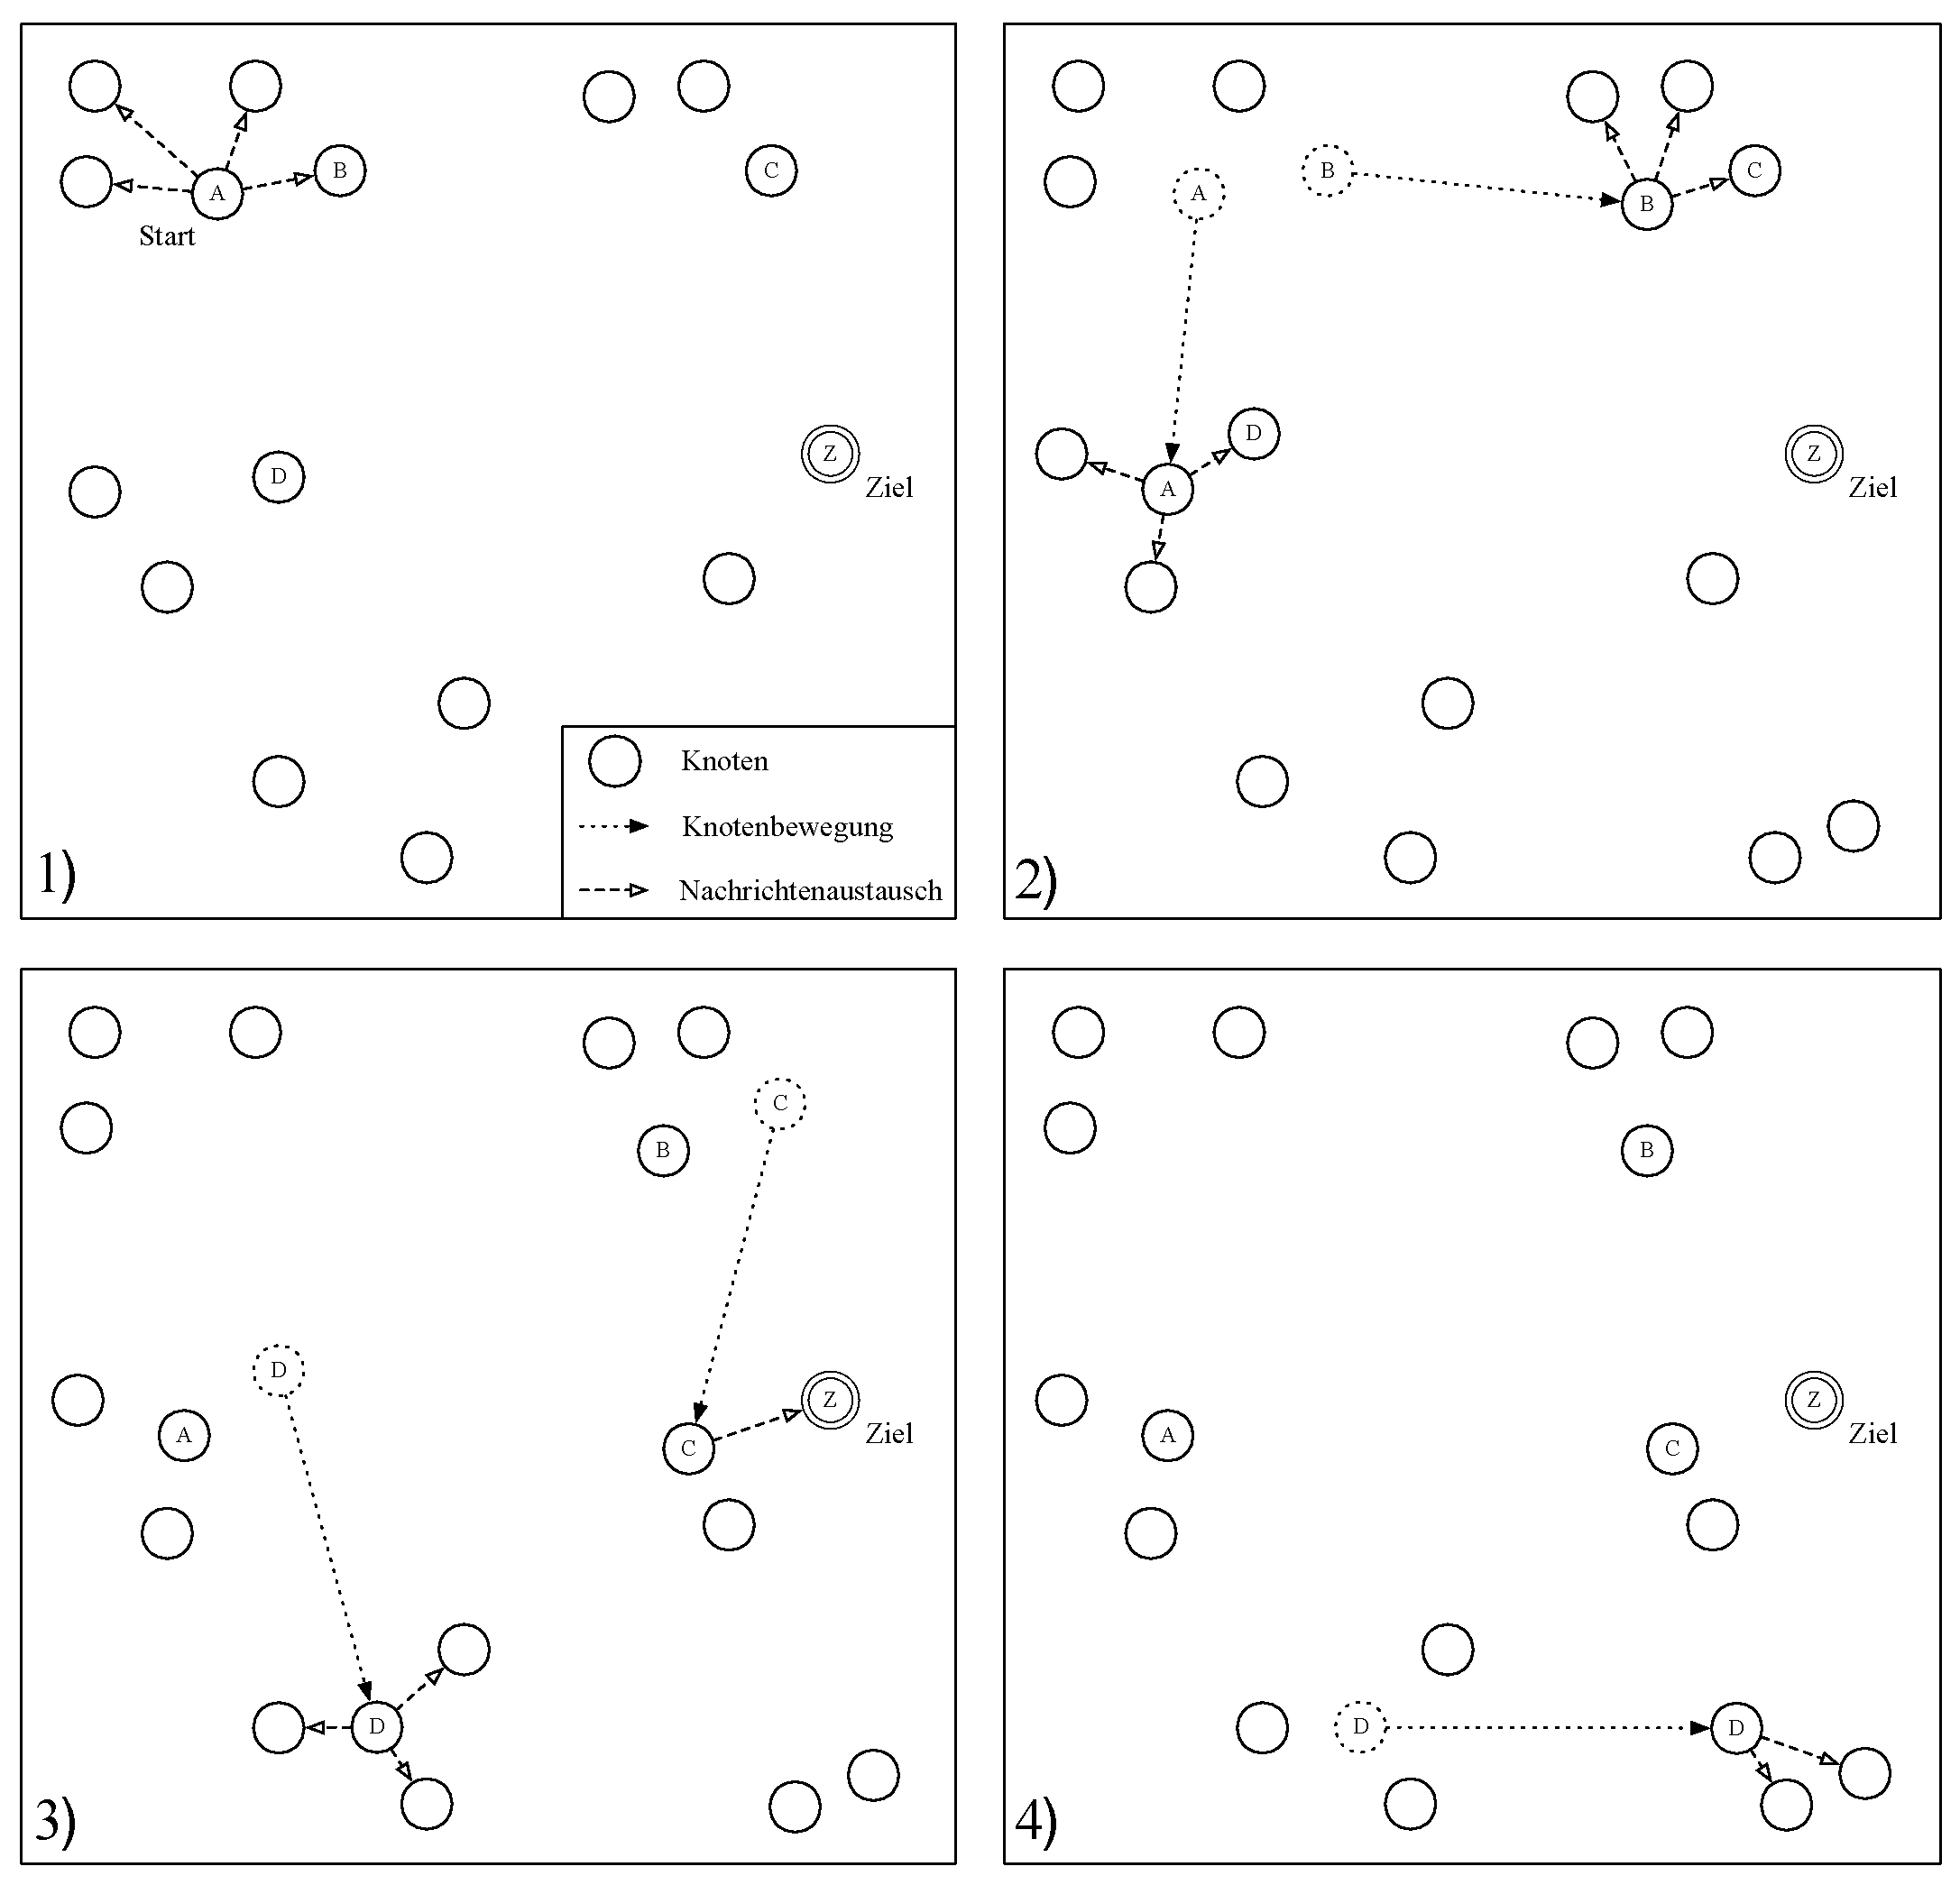
\includegraphics[width=\textwidth]{img/epidemic.pdf}
    \caption{Beispiel des Forwarding-Protokolls Epidemic. Bilder 1) - 4) stellen einzelne Zeitschritte dar.}
    \label{fig:epidemic}
\end{figure}
Das Weiterleiten einer Nachricht mit dem Forwarding-Protokoll \emph{Epidemic} \cite{vahdat2000epidemic} verhält sich ähnlich wie das Verbreiten einer Krankheit. Sobald ein Knoten eine Nachricht versenden möchte, überträgt er diese an jeden anderen Knoten, auf den er trifft. 
In Abbildung \ref{fig:epidemic} ist exemplarisch gezeigt wie Knoten $A$ eine Nachricht an Knoten $Z$ versendet. Während sich $A$ bewegt, sendet er seine Nachricht an insgesamt 7 andere Knoten. Knoten $B$ sendet die Nachricht an Knoten $C$, welcher sich zum Ziel bewegt und dort die Nachricht überträgt.

Hier ist zu sehen, dass der Ursprungsknoten $A$ niemals in die Nähe von seinem gewünschten Ziel gelangt. Zusätzlich kommt es zu keiner durchgehenden Verbindung, denn während sich die Knoten fortbewegen, muss es zu keinem Kontakt zu anderen Knoten kommen.
Es ist anzumerken, dass zur Vereinfachung der Darstellung Kontakte zu anderen Knoten nur in Gruppen stattfinden und sich lediglich die gekennzeichneten Knoten bewegen. Dies ist jedoch keine Bedingung für Epidemic-Forwarding. Außerdem ist ein Nachrichtenaustausch in der Abbildung immer nur einseitig dargestellt. Dies ist nur der Fall, sofern die Gegenseite überhaupt keine Nachrichten zu versenden hat.

Jeder Knoten besitzt einen Buffer, welcher sowohl eigene Nachrichten, als auch Nachrichten anderer Knoten speichert. Kommt es zu einem Kontakt, werden beide Buffer verglichen und es findet ein Austausch der Nachrichten statt, welche dem jeweils anderen Knoten fehlen.
Um zu verhindern, dass Nachrichten, welche evtl. bereits erfolgreich übertragen wurden, sich in anderen Teilen des Netzwerks weiter verbreiten, können ACK-Requests oder Hop-Counts implementiert werden. Beispielsweise ist in Abbildung \ref{fig:epidemic} die Nachricht von Knoten $A$ bereits erfolgreich an $Z$ übertragen, während sie jedoch von Knoten $D$ weiter verteilt wird.
Durch die Implementation eines Hop-Counts (vergleichbar mit TTL in IP) würden Nachrichten aus dem Buffer entfernt, sobald sie eine gewisse Anzahl an Übertragungen überschritten haben.
Mit einem ACK-Request, welcher vom Zielknoten in das Netzwerk gegeben wird, würden alle Knoten, welche diesen Request erhalten, die ursprüngliche Anfrage aus ihrem Buffer entfernen. Zusätzlich bekommt der Sender (falls er den ACK erhält) die Information, dass seine Nachricht erfolgreich übermittelt wurde.
% ??? vorteile nachteile von hop und ack

% Vor und nachteile
Ein Vorteil dieses Verfahrens ist die hohe Wahrscheinlichkeit, mit der Nachrichten erfolgreich an ihr Ziel gebracht werden, denn je mehr Knoten die Nachricht verbreiten, desto mehr Knoten werden damit erreicht.
Dies resultiert jedoch in einem der größten Nachteile dieses Verfahrens: Es findet mit jedem Kontakt ein Nachrichtenaustausch statt, was dazu führt, dass die in der Regel limitierte Speicherkapazität überschritten und ein weiteres Aufnehmen von Informationen somit unmöglich wird.
Durch die häufigen Datenübetragungen kristallisiert sich dieses Protokoll in manchen Anwendungen als wenig praktikabel heraus. Häufige Datentransfers sorgen neben Speicherlimitation für hohen Energieverbrauch.

Das in Abschnitt \ref{sec:applications:haggle} vorgestellte Haggle Project verwendet Epidemic-Forwarding insofern, als dass Nachrichten an \emph{alle} User geschickt werden, welche übereinstimmende Interessen besitzen. Hierbei ist jedoch zu bemerken, dass Sender und Empfänger der Daten die beiden im Kontakt beteiligten Knoten sind.

\subsection{Partieller Kontext - PRoPHET}
\emph{PRoPHET} \cite{lindgren2003probabilistic} steht für \emph{Probabilistic Routing Protocol using History of Encounters and Transitivity} und der Kern dieses Forwarding-Protokolls ist, Nachrichten nur an jene Knoten weiter zu leiten, welche mit einer gewissen Warscheinlichkeit die Nachricht bis zum Ziel bringen werden. 
Dieses Protokoll basiert auf der Annahme, dass Bewegungsmuster von Knoten nicht randomisiert sind, sondern eine gewisse Struktur aufweisen. Struktur bedeutet, dass Knoten, welche sich oft gesehen haben, sich auch in Zukunft oft sehen werden.

Wie in \cite{lindgren2003probabilistic} beschrieben, besitzt jeder Knoten $A$ eine Tabelle, in der für alle anderen Knoten $B$ ein Wert $0 \leq p(A,B) \leq 1$ eingetragen ist, welcher die Wahrscheinlichkeit einer erfolgreichen Übertragung von $A$ nach $B$ angibt. Dieser Wert wird \emph{delivery predictabilty} genannt.

In den nächsten beiden Kapiteln wird zunächst auf das Aktualisieren der Tabelle (Kapitel \ref{sec:prophet:tabellenupdate}) und anschließend auf den generellen Ablauf des Protokolls eingegangen (Kapitel \ref{sec:prophet:forwarding}).

\subsubsection{Tabellen-Update}
\label{sec:prophet:tabellenupdate}
Bei jedem Kontakt werden die Wahrscheinlichkeitstabellen ausgetauscht und es findet ein Update der Werte statt (die folgenden Gleichungen sind aus \cite{lindgren2003probabilistic} entnommen).
Zunächst wird der aktuelle Kontakt zwischen den Knoten $A$ und $B$ mithilfe des Terms (\ref{eq:updatenormal}) bewertet. Dazu wird in der Tabelle die Wahrscheinlichkeit, dass dieser Kontakt erneut auftritt erhöht.
$p(A,B)_{old}$ stellt den Wert in der Tabelle dar, welcher vor dem Kontakt existierte und $P_{init} \in (0,1]$ ist eine Konstante, welche die positive Auswirkung auf die Wahrscheinlichkeit eines erneuten Treffens reguliert. Wie $p(A,B)_{old}$ initial gewählt wird hängt vom Szenario ab.
\begin{equation}
	\label{eq:updatenormal}
	p(A,B) = p(A,B)_{old} + (1-p(A,B)_{old}) \times P_{init}
\end{equation}
Anschließend wird ein Alterungsprozess simuliert, indem jede Wahrscheinlichkeit reduziert wird, abhängig davon wie lange ein Kontakt zurückliegt. In Term (\ref{eq:updateage}) steht $\lambda \in (0,1)$ für eine Konstante, welche diesen Prozess reguliert und $k$ für die Zeiteinheiten seit der letzten Alterung.
\begin{equation}
	\label{eq:updateage}
	p(A,B) = p(A,B)_{old} \times \lambda^k
\end{equation}
In der letzten Phase des Updates werden die Daten des im Kontakt stehenden Knotens verwendet um transitive Beziehungen zu Knoten miteinzubeziehen. Das bedeutet, dass $p(A,C)$ abhängig von den Werten $p(A,B)$ und $p(B,C)$ geändert wird.
In Term (\ref{eq:updatetransversal}) stellt $\beta \in [0,1]$ eine Konstante dar, die den Einfluss der Transitivität reguliert.
\begin{equation}
	\label{eq:updatetransversal}
	p(A,C) = p(A,C)_{old} + (1-P(A,C)_{old}) \times P(A,B) \times P(B,C) \times \beta
\end{equation}
Das Festlegen jeder Konstante ist stark von dem jeweiligen Szenario, in dem das Protokoll eingesetzt wird, abhängig.

\subsubsection{Forwarding-Prozess}
\label{sec:prophet:forwarding}
Nach dem Update der jeweiligen Tabellen entscheidet das Protokoll, ob und welche Nachrichten an den anderen Knoten übertragen werden sollen. Eine Möglichkeit wäre eine Grenze $g \in (0,1)$ festzulegen, welche eine Nachrichtenübertragung herbeiführt, sobald $p(A,B) > g$. Hier ist die Schwierigkeit $g$ korrekt festzulegen, da ohne weiteres keine Aussage über die im Netz vorkommenden $p$-Werte gemacht werden kann.
Auch hier ist zu betonen, dass die jeweiligen Einstellungen stark von dem jeweiligen Anwendungsgebiet abhängen und dementsprechend gewählt werden müssen.
% ??? mehr vor und nachteile




\subsection{Voller Kontext - SimBet}
\label{sec:simbet}
Der Name des Protokolls \emph{SimBet} \cite{daly2007social} ist eine Zusammensetzung der Worte \emph{similarity} und \emph{betweenness}. Diese Ausdrücke stehen für die Metrik, die verwendet wird um eine Forwarding-Entscheidung zu treffen.
Die Idee hinter SimBet ähnelt der von PRoPHET, indem angenommen wird, dass Nutzer in einem Netzwerk eine gewisse Sozialstruktur aufweisen. Im Falle von SimBet bedeutet dies, dass sich Knoten vornehmlich in sogenannten \emph{Communities} aufhalten. Das sind Gruppen von Knoten, welche häufig miteinander verbunden sind.
In Abbildung \ref{fig:simbet} gibt es zwei Communities, eine bestehend aus $\{1,2,3,4\}$ und eine andere bestehend aus $\{5,6,7\}$.
\begin{figure}[H]
    \centering
    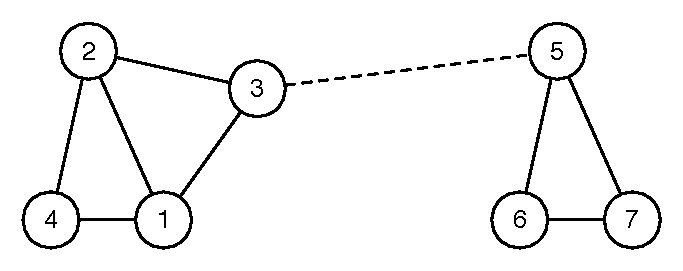
\includegraphics[width=0.5\textwidth]{img/simbet.pdf}
    \caption{Beispiel einer Beziehungskonstellation in SimBet}
    \label{fig:simbet}
\end{figure}
Die zum Forwarding verwendete Metrik $SimBetUtil_n(d)$, die ein Maß dafür gibt, wie gut sich ein Knoten $n$ als nächster Hop zum Zielknoten $d$ eignet, besteht aus dem \emph{Betweenness-} und dem \emph{Similarity-Index}.
Der Betweenness-Index sagt aus, wie stark ein Knoten die eigene Nachbarschaft an andere Nachbarschaften anknüpft. Der Similarity-Index gibt Auskunft darüber, wie ähnlich die Nachbarschaft eines Knotens zu der des Zielknotens ist.
Der Ablauf lässt sich wie folgt darstellen: Zunächst versucht SimBet eine Nachricht mithilfe des Betweenness-Index in die Community des Zielknotens weiterzuleiten. Anschließend wird innerhalb der Community die Nachricht mithilfe des Similarity-Index zum Zielknoten weitergeleitet.
Mathematisch lässt sich diese Vorschrift in (\ref{eq:simbetutil}) ablesen. Die Konstanten $\alpha$ und $\beta$ regulieren den Einfluss, den der Similarity- bzw. der Betweenness-Index auf die Berechnung hat.
\begin{equation}
	\label{eq:simbetutil}
	SimBetUtil_n(d) = \alpha Sim_n(d) + \beta Bet_n(d) \quad \text{mit} \quad 1=\alpha + \beta
\end{equation}

\subsubsection{Betweenness-Index}
Jeder Knoten besitzt eine Matrix, in der die direkten Nachbarn eingetragen sind. In (\ref{eq:k2}) sind zwei Matrizen exemplarisch aufgeführt, welche die Nachbarschaftsstrukturen der Knoten $2$ und $3$ aus Abbildung \ref{fig:simbet} darstellen. Wenn $a_{i,j} = 1$, existiert eine direkte Verbindung zwischen den Knoten $i$ und $j$.
\begin{equation}
	\label{eq:k2}
	N_{k_2} = \bordermatrix{~ 	& k_1	& k_2	& k_3	& k_4 \cr
                  		k_1 & 0 	& 1 	& 1 	& 1 \cr
                  		k_2 & 1 	& 0 	& 1 	& 1 \cr
                  		k_3 & 1 	& 1 	& 0 	& 0 \cr
                  		k_4 & 1 	& 1 	& 0 	& 0 \cr}
                  		\quad \quad \quad \quad
    N_{k_3} = \bordermatrix{~ 	& k_1	& k_2	& k_3	& k_5 \cr
                  		k_1 & 0 	& 1 	& 1 	& 0 \cr
                  		k_2 & 1 	& 0 	& 1 	& 0 \cr
                  		k_3 & 1 	& 1 	& 0 	& 1 \cr
                  		k_5 & 0 	& 0 	& 1 	& 0 \cr}
\end{equation}
Mithilfe des Betweenness-Index kann das Protokoll entscheiden, wie gut eine Nachricht zwischen den Communities transportiert werden kann. 
Betrachte man den Knoten $3$ aus Abbildung \ref{fig:simbet}, so ist für die Berechnung des Index wichtig, wieviele Verbindungen $c$ Knoten $3$ zu anderen Knoten hat, die Knoten $1$ und $2$ nicht haben. Je größer also $c$, desto größer ist auch der Betweenness-Index. 
%In der obigen Abbildung lässt sich erkennen, dass Knoten $3$ die einzige Verbindung zu der anderen Community ist. Die Knoten $1$ und $2$ verfügen nicht über diesen Link.
\\
Die genauen mathematischen Formeln sind in \cite[p.~35f]{daly2007social} nachzulesen.
% \begin{align}
% 	(k_3)^2[1-k_3] &= 
% 	\begin{pmatrix}
% 	  0 & 1 & 1 & 0  \\
% 	  1 & 0 & 1 & 0  \\
% 	  1 & 1 & 0 & 1  \\
% 	  0 & 0 & 1 & 0
%  	\end{pmatrix}
%  	*
%  	\begin{pmatrix}
% 	  0 & 1 & 1 & 0  \\
% 	  1 & 0 & 1 & 0  \\
% 	  1 & 1 & 0 & 1  \\
% 	  0 & 0 & 1 & 0
%  	\end{pmatrix}
%  	\left [1-
%  	\begin{pmatrix}
% 	  0 & 1 & 1 & 0  \\
% 	  1 & 0 & 1 & 0  \\
% 	  1 & 1 & 0 & 1  \\
% 	  0 & 0 & 1 & 0
%  	\end{pmatrix} 
%  	\right ]
%  	\\
%  	&=
%  	\begin{pmatrix}
% 	 2 & 1 & 1 & 1 \\
% 	 1 & 2 & 1 & 1 \\
% 	 1 & 1 & 3 & 0 \\
% 	 1 & 1 & 0 & 1 \\
%  	\end{pmatrix}
%  	\left [
%  	\begin{pmatrix}
% 		1 & 0 & 0 & 1 \\
% 		0 & 1 & 0 & 1 \\
% 		0 & 0 & 1 & 0 \\
% 		1 & 1 & 0 & 1 \\
%  	\end{pmatrix} 
%  	\right ]
%  	\\
%  	&=
%  	\begin{pmatrix}
% 	 2 & 0 & 0 & 1 \\
% 	 0 & 2 & 0 & 1 \\
% 	 0 & 0 & 3 & 0 \\
% 	 1 & 1 & 0 & 1 \\
%  	\end{pmatrix}
% \end{align}

\subsubsection{Similarity-Index}
Die Berechnung des Similarity-Index wird durch Vergleich der Einträge einer Reihe in der Matrix erstellt.
Betrachte man die Matrix $N_{k_3}$ in (\ref{eq:k2}), so hat $k_1$ einen gleichen Eintrag, $k_2$ einen gleichen Eintrag und $k_5$ keinen gleichen Eintrag mit $k_3$. Am Beispiel betrachtet bedeutet dies, dass $k_3$ einen Knoten mit $k_1$, einen Knoten mit $k_2$ und keinen Knoten mit $k_5$ gemein hat.
Im Forwarding wird diese Größe dazu verwendet um innerhalb der Community eine sinnvolle Route zum Ziel zu finden. Als nächster Hop werden vornehmlich Knoten ausgewählt, welche mit dem Zielknoten eine ähnliche Nachbarschaftsstruktur aufweisen. So kann sichergestellt werden, dass der nächste Hop Kontakt zu einem Knoten hat, welcher dem Ziel ein Stück näher ist.\\
Auch hier wird für die genauen Berechnungen auf \cite[p.~35f]{daly2007social} verwiesen.


\section{Bewegungsmodelle}
\label{sec:simulation}
Um die Performance eines Protokolls zu zu evaluieren ist es notwendig dieses zu testen. Da OppNets aus mobilen Knoten bestehen, müssen den Knoten Bewegungsmuster zugeteilt werden. Aus den Bewegungen werden Daten gewonnen, wie die Anzahl, die Dauer oder die Beteiligten von Kontakten.
Die Bewegungsmuster können entweder durch Messungen gesammelt, oder künstlich berechnet worden sein \cite{Mota20145}.

Messungen von Knotenbewegungen haben den Vorteil, dass sie die realen Bewegungen der Knoten in einem gewissen Szenario wiedergeben. Eine synthetische Generierung der Daten hingegen kann niemals dieselbe Güte an Realität bieten.
Auf der anderen Seite ist die Menge an existierenden Messungen begrenzt. Daraus entsteht das Problem, dass nicht alle Messungen passend für das jeweilige Szenario sind. So stellen Messungen von Menschenbewegungen eine schlechte Grundlage zur Auswertung eines OppNets dar, welches für die Kommunikation zwischen Autos verwendet wird.
Aufgrund der Vielzahl unterschiedlicher Protokollarten werden daher häufig synthetisch generierte Bewegungsmodelle zur Simulation verwendet.

Im Folgenden werden zwei synthetische Bewegungsmodelle vorgestellt.

\subsection{Random Walk Mobility Model}
Das \emph{Random Walk Mobility Model} \cite{roy2011random} ist ein simples Bewegungsmodell, in der ein Knoten von seiner aktuellen Position randomisiert eine Richtung und eine Geschwindigkeit festlegt, mit der er sich zur nächsten Position bewegt. Dieses Modell ist ein sogenanntes \emph{Entity Mobility Model}, was bedeutet, dass lediglich die Bewegungen eines einzelnen Knotens in Betracht gezogen werden.
Die Entfernung, die der Knoten zurücklegt, ist entweder durch eine feste Zeitdauer oder durch eine feste Entfernung festgelegt.
Dieser Prozess findet an jeder erreichten Position erneut statt. Sollten Knoten an das Ende der Simulationsfläche kommen, werden sie wieder zurück reflektiert.
Regulieren lässt sich das Model in der Anzahl seiner Knoten, der Größe der Fläche, auf der sich die Knoten bewegen, dem Geschwindigkeitsbereich und in den zugelassenen Winkeln.
\begin{figure}[H]
    \centering
    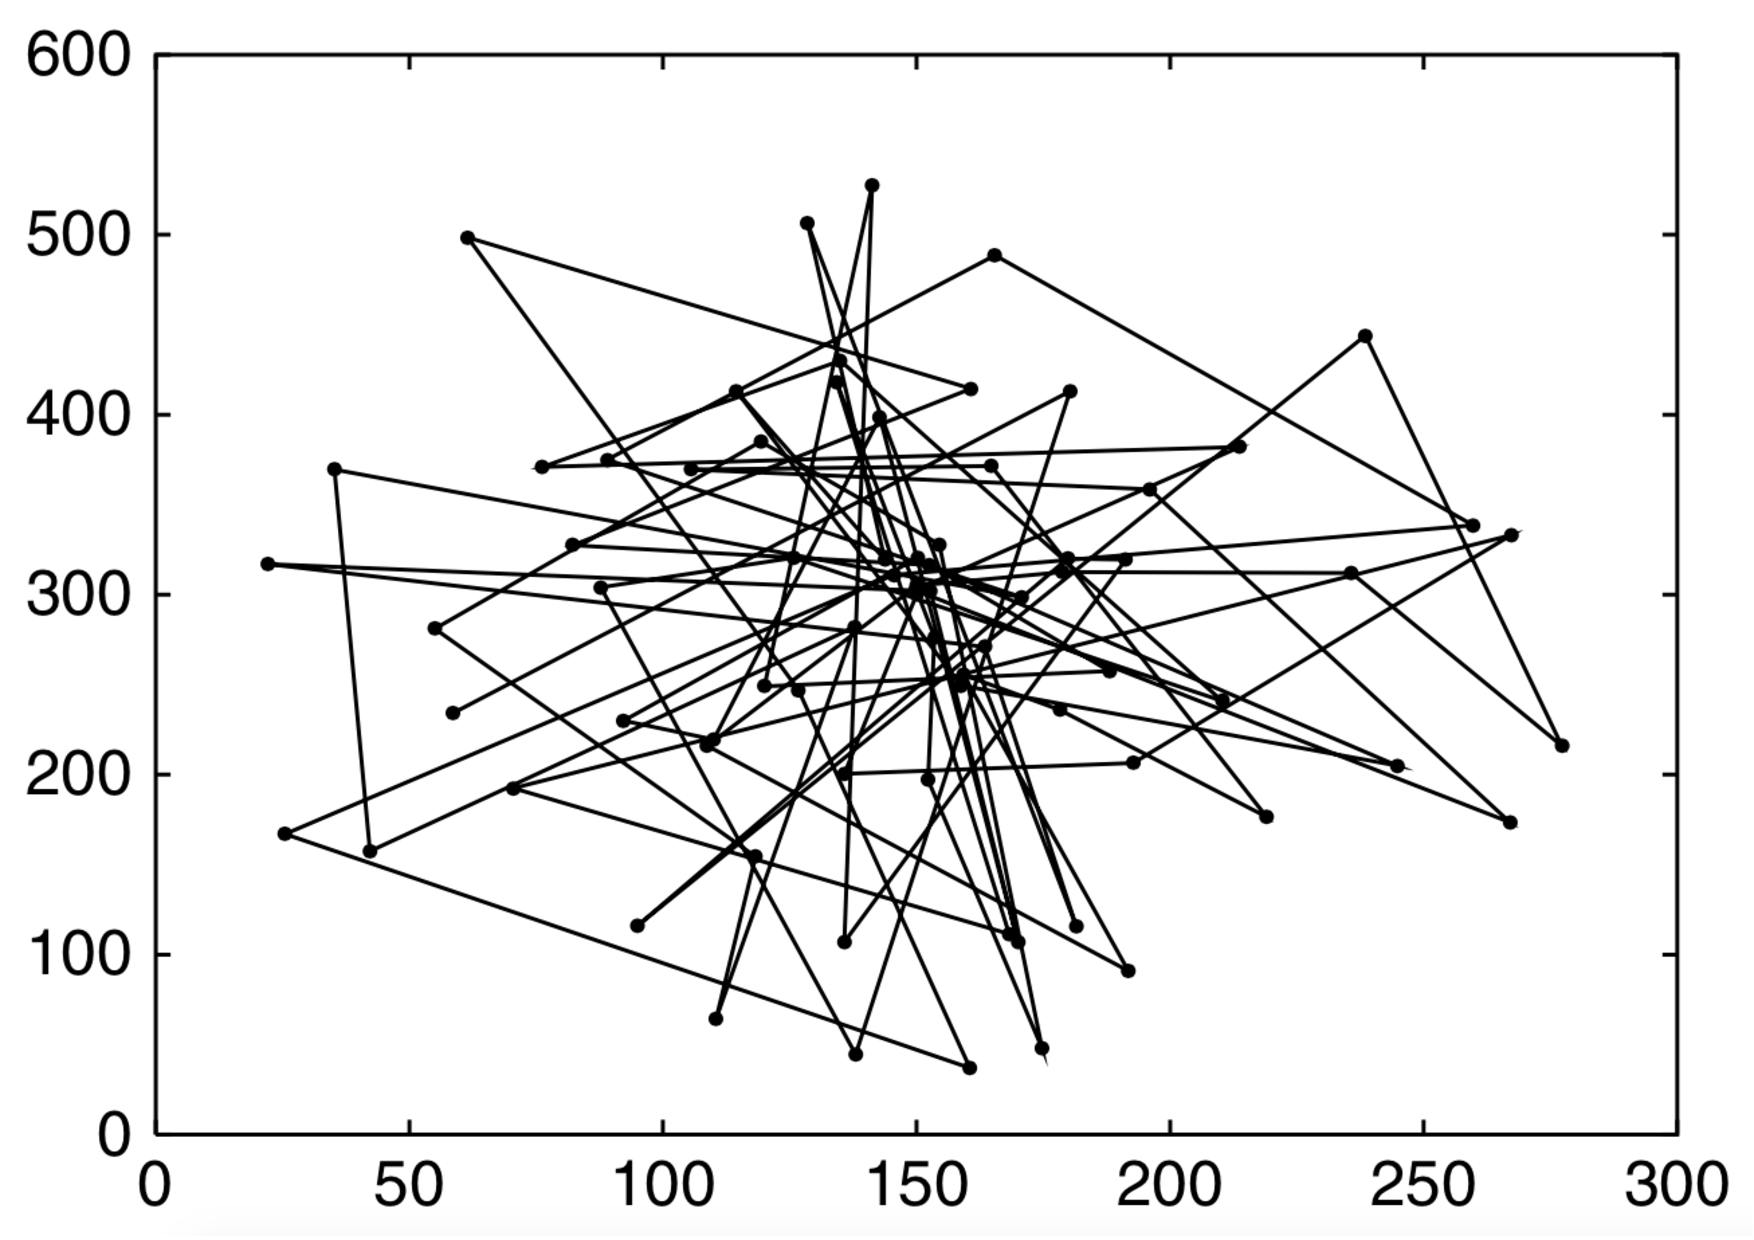
\includegraphics[width=0.4\textwidth]{img/randomW.pdf}
    \caption{Zeigt das Random Walk Bewegungsmuster eines Knotens. 
    \textbf{Quelle:} \cite{roy2011random}}
    \label{fig:randomwaypoint}
\end{figure}

In Abbildung \ref{fig:randomwaypoint} ist das Random Walk Bewegungsmuster eines Knotens dargestellt. Nach jeder Geschwindigkeits- und Richtungsneuberechnung bewegt sich der Knoten für 60s lang in eine Richtung.
Es ist zu erkennen, dass die Bewegungsrichtungen teilweise extrem spitze Winkel aufweisen. Dies liegt an der zufälligen Auswahl der Richtung, welche keinen Bezug zu den bereits zurückgelegten Wegen haben.

\subsection{Pursue Mobility Model}
Wie in Abschnitt \ref{sec:simbet} zu sehen ist, arbeiten Protokolle wie SimBet auf Basis des Gruppenverhaltens der Knoten. Dies muss in den Simulationen berücksichtigt werden und erfordert somit Bewegungsmodelle, die Gruppendynamik beachten.
\begin{figure}[H]
    \centering
    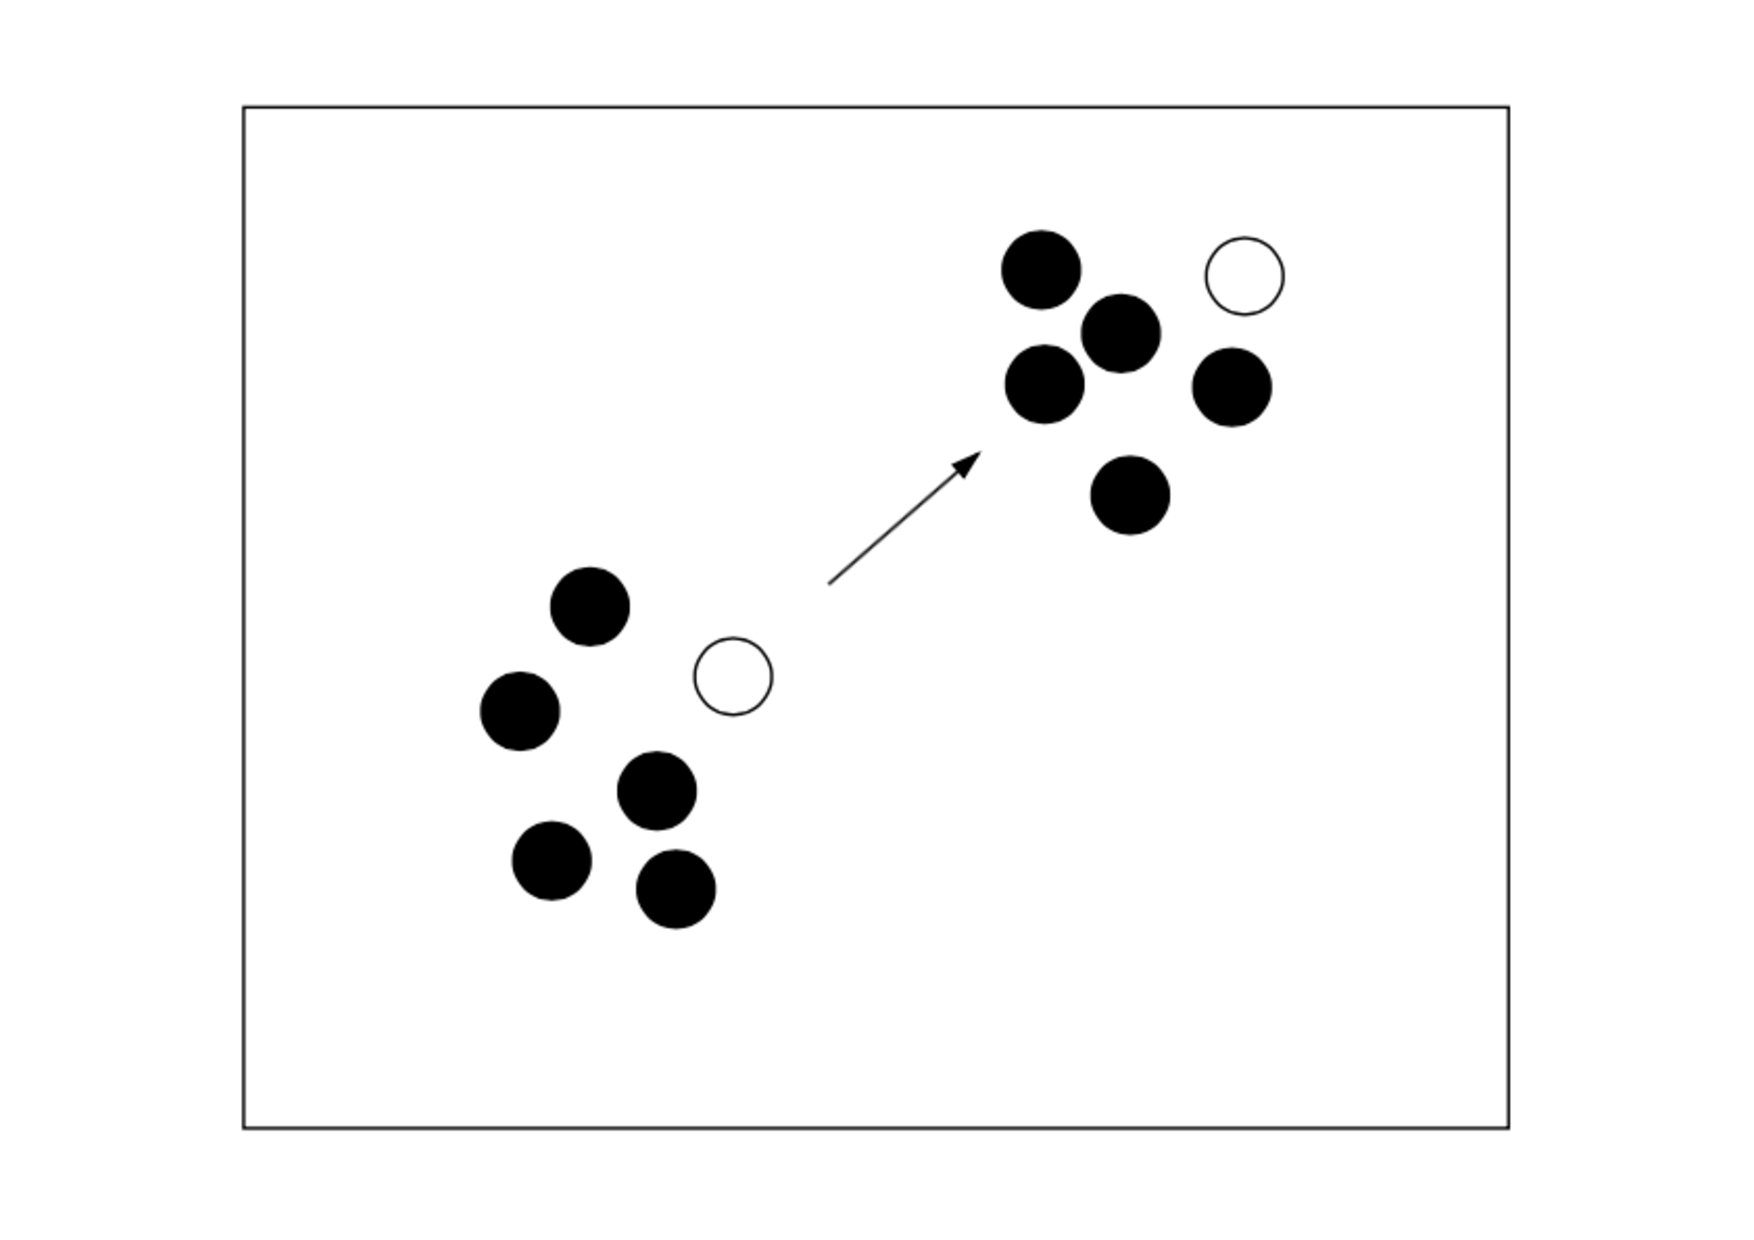
\includegraphics[width=0.4\textwidth]{img/pursue.pdf}
    \caption{Zeigt die Gruppenbewegung des Pursue Mobility Model. \textbf{Quelle:} \cite{camp2002survey}}
    \label{fig:pursue}
\end{figure}
Das \emph{Pursue Mobility Model} \cite{camp2002survey} ist ein \emph{Group Mobility Model}, da es Gruppenbewegungen modelliert.
Die Idee hinter diesem Modell ist, dass eine Gruppe von Knoten ein Ziel verfolgt. Dabei stellt das Ziel meist ein anderer Knoten dar.
In Abbildung \ref{fig:pursue} ist zu sehen, wie eine Gruppe von schwarzen Knoten einen weißen Knoten verfolgt. 
Neben dem Verfolgen des weißen Knotens haben die schwarzen Knoten eine zufällige Komponente mit der sie sich in einem gewissen Radius selber bewegen dürfen.
In Gleichung (\ref{eq:pursue}) wird diese Komponente durch $random\_vector$ ausgedrückt, welcher z.B. mithilfe des Random Walk Mobility Models erstellt werden kann.
\begin{equation}
	\label{eq:pursue}
	\text{newPosition} = \text{oldPosition} + \text{acceleration}(\text{target} - \text{oldPosition}) + \text{randomVector}
\end{equation}
Die Funktion $\text{acceleration}(\text{target}-\text{oldPosition})$ berechnet aus dem verfolgten Ziel und der aktuellen Position die neue Richtung, in die gegangen werden soll.



% \section{Probleme und Fragestellungen}
% \label{sec:problems}
% %    evtl
% Hervorheben des Forschungsfortschritts. Darauf aufbauend Problematik von Vergleichbarkeit(simulatoren), verschweigen von Dingen(Energie), etc. aufzeigen.
% Probleme beim evaluieren der protokolle, weil sehr anwendungsabhängig...ich möchte eine simulation erstellen, welche communities mapt? will ichd as?
% Die frage ist, wie sich menschen/tiere verhalten..also patterns herausfinden.
% Netzabdeckung?

\section{Zusammenfassung}
\label{sec:conclusion}
% Mit dieser
% Zunächst wird die Arbeit samt ihrer Fragestellung zusammengefasst.
% Ich könnte hier auch noch meine Meinung kundtun, falls ich den Forschungszustand irgendwie interessant zu WOrten bringen könnte.
% Ausblick bietet sich bei einem Überblickspaper eher nicht an, weil man sich ja überall hin ausblicken müsste...
Im Rahmen dieser Ausarbeitung sollen die Grundlagen des Bereichs der opportunistischen Netze vermittelt werden. Zunächst wurde der Begriff der  opportunistischen Netze erläutert und in einen Kontext gebracht. Anschließend wurden Beispiele gegeben in denen OppNets verwendet vorkommen. Danach wurde ein Einblick in verschiedene Forwarding-Strategien gegeben. Daraufhin wurden Bewegungsmodelle vorgestellt, welche zur Messung der Performance von OppNets verwendet werden können.


% Bibliography
\bibliographystyle{ieeetr}
\bibliography{oppnet}
\end{document}